% Options for packages loaded elsewhere
\PassOptionsToPackage{unicode}{hyperref}
\PassOptionsToPackage{hyphens}{url}
\PassOptionsToPackage{dvipsnames,svgnames,x11names}{xcolor}
%
\documentclass[
  authoryear,
  preprint,
  3p]{elsarticle}

\usepackage{amsmath,amssymb}
\usepackage{lmodern}
\usepackage{iftex}
\ifPDFTeX
  \usepackage[T1]{fontenc}
  \usepackage[utf8]{inputenc}
  \usepackage{textcomp} % provide euro and other symbols
\else % if luatex or xetex
  \usepackage{unicode-math}
  \defaultfontfeatures{Scale=MatchLowercase}
  \defaultfontfeatures[\rmfamily]{Ligatures=TeX,Scale=1}
\fi
% Use upquote if available, for straight quotes in verbatim environments
\IfFileExists{upquote.sty}{\usepackage{upquote}}{}
\IfFileExists{microtype.sty}{% use microtype if available
  \usepackage[]{microtype}
  \UseMicrotypeSet[protrusion]{basicmath} % disable protrusion for tt fonts
}{}
\makeatletter
\@ifundefined{KOMAClassName}{% if non-KOMA class
  \IfFileExists{parskip.sty}{%
    \usepackage{parskip}
  }{% else
    \setlength{\parindent}{0pt}
    \setlength{\parskip}{6pt plus 2pt minus 1pt}}
}{% if KOMA class
  \KOMAoptions{parskip=half}}
\makeatother
\usepackage{xcolor}
\setlength{\emergencystretch}{3em} % prevent overfull lines
\setcounter{secnumdepth}{5}
% Make \paragraph and \subparagraph free-standing
\ifx\paragraph\undefined\else
  \let\oldparagraph\paragraph
  \renewcommand{\paragraph}[1]{\oldparagraph{#1}\mbox{}}
\fi
\ifx\subparagraph\undefined\else
  \let\oldsubparagraph\subparagraph
  \renewcommand{\subparagraph}[1]{\oldsubparagraph{#1}\mbox{}}
\fi


\providecommand{\tightlist}{%
  \setlength{\itemsep}{0pt}\setlength{\parskip}{0pt}}\usepackage{longtable,booktabs,array}
\usepackage{calc} % for calculating minipage widths
% Correct order of tables after \paragraph or \subparagraph
\usepackage{etoolbox}
\makeatletter
\patchcmd\longtable{\par}{\if@noskipsec\mbox{}\fi\par}{}{}
\makeatother
% Allow footnotes in longtable head/foot
\IfFileExists{footnotehyper.sty}{\usepackage{footnotehyper}}{\usepackage{footnote}}
\makesavenoteenv{longtable}
\usepackage{graphicx}
\makeatletter
\def\maxwidth{\ifdim\Gin@nat@width>\linewidth\linewidth\else\Gin@nat@width\fi}
\def\maxheight{\ifdim\Gin@nat@height>\textheight\textheight\else\Gin@nat@height\fi}
\makeatother
% Scale images if necessary, so that they will not overflow the page
% margins by default, and it is still possible to overwrite the defaults
% using explicit options in \includegraphics[width, height, ...]{}
\setkeys{Gin}{width=\maxwidth,height=\maxheight,keepaspectratio}
% Set default figure placement to htbp
\makeatletter
\def\fps@figure{htbp}
\makeatother

\usepackage{booktabs}
\usepackage{longtable}
\usepackage{array}
\usepackage{multirow}
\usepackage{wrapfig}
\usepackage{float}
\usepackage{colortbl}
\usepackage{pdflscape}
\usepackage{tabu}
\usepackage{threeparttable}
\usepackage{threeparttablex}
\usepackage[normalem]{ulem}
\usepackage{makecell}
\usepackage{xcolor}
\makeatletter
\makeatother
\makeatletter
\makeatother
\makeatletter
\@ifpackageloaded{caption}{}{\usepackage{caption}}
\AtBeginDocument{%
\ifdefined\contentsname
  \renewcommand*\contentsname{Table of contents}
\else
  \newcommand\contentsname{Table of contents}
\fi
\ifdefined\listfigurename
  \renewcommand*\listfigurename{List of Figures}
\else
  \newcommand\listfigurename{List of Figures}
\fi
\ifdefined\listtablename
  \renewcommand*\listtablename{List of Tables}
\else
  \newcommand\listtablename{List of Tables}
\fi
\ifdefined\figurename
  \renewcommand*\figurename{Figure}
\else
  \newcommand\figurename{Figure}
\fi
\ifdefined\tablename
  \renewcommand*\tablename{Table}
\else
  \newcommand\tablename{Table}
\fi
}
\@ifpackageloaded{float}{}{\usepackage{float}}
\floatstyle{ruled}
\@ifundefined{c@chapter}{\newfloat{codelisting}{h}{lop}}{\newfloat{codelisting}{h}{lop}[chapter]}
\floatname{codelisting}{Listing}
\newcommand*\listoflistings{\listof{codelisting}{List of Listings}}
\makeatother
\makeatletter
\@ifpackageloaded{caption}{}{\usepackage{caption}}
\@ifpackageloaded{subcaption}{}{\usepackage{subcaption}}
\makeatother
\makeatletter
\@ifpackageloaded{tcolorbox}{}{\usepackage[many]{tcolorbox}}
\makeatother
\makeatletter
\@ifundefined{shadecolor}{\definecolor{shadecolor}{rgb}{.97, .97, .97}}
\makeatother
\makeatletter
\makeatother
\journal{Journal of Behavioral and Experimental Economics}
\ifLuaTeX
  \usepackage{selnolig}  % disable illegal ligatures
\fi
\usepackage[]{natbib}
\bibliographystyle{elsarticle-harv}
\IfFileExists{bookmark.sty}{\usepackage{bookmark}}{\usepackage{hyperref}}
\IfFileExists{xurl.sty}{\usepackage{xurl}}{} % add URL line breaks if available
\urlstyle{same} % disable monospaced font for URLs
\hypersetup{
  pdftitle={Revisiting `Growth and Inequality in Public Good Provision' ---Reproducing and Generalizing Through Inconvenient Online Experimentation},
  pdfauthor={Hauke Roggenkamp},
  pdfkeywords={Replication study, Non-convenience sample, Open
science, Dynamic public goods game, Online
experiment, Generalizability},
  colorlinks=true,
  linkcolor={blue},
  filecolor={Maroon},
  citecolor={Blue},
  urlcolor={Blue},
  pdfcreator={LaTeX via pandoc}}

\setlength{\parindent}{6pt}
\begin{document}

\begin{frontmatter}
\title{Revisiting `Growth and Inequality in Public Good Provision'
---Reproducing and Generalizing Through Inconvenient Online
Experimentation}
\author[1,2]{Hauke Roggenkamp%
%
}
 \ead{hauke.roggenkamp@unisg.ch} 

\affiliation[1]{organization={Helmut Schmidt
University},addressline={Holstenhofweg
85},city={Hamburg},postcode={22043}}
\affiliation[2]{organization={University of
St.~Gallen},addressline={Torstrasse
25},city={St.~Gallen},postcode={9000}}

\cortext[cor1]{Corresponding author}

        
\begin{abstract}
I revisit the dynamic public goods game developed by Gächter et
al.~(2017) to study cooperation under dynamic interdependencies.
Collecting data from both a convenient (students) and an inconvenient
(general population) sample, I not only reproduce some of the author's
original observations but also test their novel game's generalizability.
Appending a charitable dictator game, I find no correlations between
behavior in the charitable context and the dynamic game. This applies to
students and the general population sample alike. Because the study of
inexperiend general population samples raises methodological challenges,
such as fatigue and dropouts, this research approaches them. Doing so, I
provide simple solutions to run relieable interactive experiments
online.

You can find the most recent version of this paper
\href{https://github.com/Howquez/coopUncertainty/blob/main/analysis/quarto/paper.pdf}{here}.
\end{abstract}





\begin{keyword}
    Replication study \sep Non-convenience sample \sep Open
science \sep Dynamic public goods game \sep Online experiment \sep 
    Generalizability
\end{keyword}
\end{frontmatter}\ifdefined\Shaded\renewenvironment{Shaded}{\begin{tcolorbox}[enhanced, borderline west={3pt}{0pt}{shadecolor}, breakable, boxrule=0pt, interior hidden, sharp corners, frame hidden]}{\end{tcolorbox}}\fi

\hypertarget{sec-intro}{%
\section{Introduction}\label{sec-intro}}

Today's actions are tomorrow's result. There are many settings in which
current decisions affect future outcomes and with it, future decision
spaces. Opting for environmental friendly policies today not only
reduces carbon dioxide omissions immediately but also helps us to reach
the Paris climate targets tomorrow. Deferring these policies, may not
necessarily prevent us from reaching these targets, but it requires more
effort in the future compared to a path that includes immediate action.
Aiming at certain goals, today's actions (or the omission thereof) not
only affect intermediate outcomes but also the number of paths one can
choose from that lead to that specific goal.

Public good (or public bad) games---although often intended to inform
climate policies
\citep[e.g.][]{MilinskiEtAl2006, TavoniEtAl2011, Hauser2014, BrickEtAl2015, GomezEtAl2018, CalzolariEtAl2018, CookEtAl2019}---miss
these temporal interdependencies simply because participants have the
same set of actions in each period. Accordingly, participants' actions
in a given period do not affect their action space in subsequent
periods. To see the lack of realism, consider carbon dioxide emissions,
where the current stock will last for well over a millennium
\citep{Inman2008, CalzolariEtAl2018}. Playing with fresh endowments in
each period is as if one could just undo carbon dioxide emissions at no
cost.

A game designed by Gächter, Mengel, Tsakas \& Vostroknutov \citeyearpar[
hereafter, GMTV]{GMTV2017} as well as Stefan Große (2011, unpublished)
shows that it is fairly simple to remedy that limitation. They
incorporated interdependencies into a \emph{dynamic} public goods game
(dPGG) by defining endowments as the income of previous periods. To put
it differently, participants' actions in a given period affect their
number of actions in subsequent periods: the more (less) they earn now,
the more (less) they can contribute in the next period. Importantly,
this modification qualitatively yields the same rational predictions as
the static game (i.e.~free-riding and the under-provision of the public
good). It is thus, equally well suited to study dilemma situations.

Because there is surprisingly little experimental research on
interdependencies\footnote{One exemption are \citet{Moser2019}, who
  built on GMTV's design to investigate leadership.}, I reproduced one
of GMTV's treatments to compare dynamics across (in)experienced samples
to investigate its generalizability. \citet{GKLS2020} find that static
public goods games do not generalize well to real-world climate action.
They also find that generalizability depends on structural resemblance
of the public goods game with the context of climate change mitigation:
Greater resemblance improves generalizability. Because GMTV's dynamic
setting has a more realistic property---namely, interdependencies---one
would expect it to be better suited to inform public policy. To test
this intuition, I not only ran the experiment with different samples but
also observed the participants' behavior in voluntary climate actions
(VCA).\footnote{The VCA is a (charitable) dictator game where each
  participant is a dictator dividing her budget between herself and some
  organization linked to the reduction of CO2 emissions.
  \citet{EckelGrossman1996} were the first to implement a charitable
  dictator game observing contributions of 30\% of the endowments. Like
  \citet{GKLS2020}, \citet{CarpenterEtAl2008} report that students make
  lower contributions to charity than community members.} This yielded a
setting similar to \citet{GKLS2020}'s which allows me to analyze how
behavior in the abstract game translates into real-world action across
samples. This research shows that the dynamic setting \emph{does not}
add any advances with respect to generalizability of results.

\citet{AGM2018} conducted static public goods games in the lab and on
MTurk to draw lessons from online experimentation. This study extends
this literature \citep[see,
e.g.,][]{SnowbergYariv_2021, GuptaRigottiWilson_2021, GoodmanPaolacci2017, AmirEtAl2012}
by focusing on an \emph{inconvenient} sample (i.e.~one that is
completely inexperienced sample that has not been exposed to interactive
experiments before) playing a computationally more complex game. This
required me to design a robust (and thus, more complex) software to
minimize attrition. I collected paradata to assess the desired fluency
and feasibility of the experiment. This research reports on the robust
design that made the dynamic game feasible.

Taken together, this study makes three contributions. First, it
reproduces parts of GMTV's original experiment and highlights the
importance of pure replications. Second, it shows that logistically
complex online experiments are feasible for samples other than students
or clickworkers. Third, this paper supports critics arguing that
findings from abstract games do not generalize well---not even with a
more representative sample.

After commenting on transparent research practices and reporting the
methods in Section~\ref{sec-transparency} and Section~\ref{sec-methods},
this paper is organized along these findings: The confirmatory
reproduction is reported in Section~\ref{sec-replication}, the online
feasibility in Section~\ref{sec-feasibility} and the generalizability in
Section~\ref{sec-generalizability}. Section~\ref{sec-conclusion}
concludes. Because I observed some differences in reproducing GMTV's
analysis using their data, I report these in the
\href{@sec-appendix}{Appendix}.

\hypertarget{sec-transparency}{%
\section{Transparency}\label{sec-transparency}}

Well before credibility crises comprised a variety disciplines,
\citet[p.~2]{bemwriting} indirectly conceded discrepancies between fuzzy
research processes and the polished article that results from it:

\begin{quote}
\emph{There are two possible articles you can write: (a) the article you
planned to write when you designed your study or (b) the article that
makes the most sense now that you have seen the results. They are rarely
the same, and the correct answer is (b).}
\end{quote}

Now, 20 years later, we accustom ourselves with mechanisms designed to
unravel the fuzzy back-and-forth between exploratory and confirmatory
research. Prominently, pre-registrations were established to tie the
researchers' hands when doing confirmatory research--reducing observable
discrepancies between Daryl Bem's above-mentioned (a) and (b). Today,
researchers can not only choose where to pre-register but also decide
about the level of detail they provide. More severely, nothing stops
researchers from pre-registering multiple hypotheses opposing each other
\citetext{\citealp[see, e.g.,][]{SimmonsEtAl2021}; \citealp[and][ for a
discussion]{PhamEtAl2021}}.

\citet{WaldronAllen2022} report a wide variety of depth of
pre-registrations in the field of Neuropsychopharmacology and document
that the \emph{`pre-registered'} label can be obtained with minimal
effort. In absence of transparency and scrutiny pre-registrations run
into danger to miss the target of making science more credible. Even
more so, they may have adverse effects as the \emph{`pre-registered'}
label becomes cheap (too) to acquire.

Discussing the costs and benefits of pre-registrations,
\citet{Olken2015} stresses the uncertainty of research processes and
promotes moderate approaches. As \citet{WaldronAllen2022}, he argues
that pre-registrations not necessarily eliminate flexibility. These
`moderate' or `flexible' approaches require transparency to reduce
concerns of \emph{`data-mining'} \citep[ p.~61]{Olken2015} by showing
(a) the analyses I planned to run, (b) the analysis that made most sense
after collecting the data and the transition from (a) to (b). Because
this is neither incentivized nor easy to verify, we need tools that make
transparency convenient to establish and to scrutinize. I propose
version control (such as Git) as one such tool and illustrate its
application on this paper: GitHub is a website and cloud-based service
where developers---and researchers alike---can store and manage their
code. The service is based on Git\footnote{Git is a specific open-source
  version control system developed in 2005.} and designed for version
control. Importantly, changes are time-stamped and can be tracked.
Moreover, one can create branches, that is, duplicates of code either to
work collaboratively or to archive a certain state.

To sum up, pre-registrations alone are necessary but not sufficient to
restore the credibility in experimental sciences. Pre-registrations must
come with additional emphasis on transparency covering the whole
research process as well as with a higher level of scrutiny that looks
beyond mere labels.

In fact, the experiment reported in this article qualifies for the
\emph{`pre-registered'} label at a first glance: The analysis was
pre-registered in the American Economic Association's RCT Registry
\citep{preregistration}. Further, I pre-registered the exact analyses I
planned to run when I designed the experiment on
\href{https://shorturl.at/bAGKY}{GitHub}.\footnote{https://shorturl.at/bAGKY
  to run the code, you need to execute the .Rmd files in this repository
  in the order that is indicated by file names.}

At a second glance, the analysis that made the most sense after having
collected the data and that is reported here is a little different
though: Because the more representative subject pool was exhausted
earlier than expected, I recruited students which opened up a new
research direction: assessing generalizability. Hence, this article
combines both confirmatory as well as exploratory research.

Accordingly, I edited many of the analyses scripts.\footnote{The source
  code of this document contains the analysis and can be found
  \href{https://github.com/Howquez/coopUncertainty/blob/main/analysis/quarto/paper.qmd}{here}:
  https://shorturl.at/ilpAG} However, because the originally planned
analysis code is archived and reproducible, these changes are
transparent. Importantly, I followed a literate programming approach
\citep{Knuth_1984, AkhtarYe_2023}. Hence, all documents needed to
analyze the data and to write the report stem from the same source. This
establishes consistence between the commands one tells the statistical
software to do and the explanation one tells human beings one told the
statistical software to do. As such, (a), (b) and the transition from
(a) to (b) are not only transparent but also comprehensible.

\hypertarget{sec-methods}{%
\section{Methodology}\label{sec-methods}}

In the terminology of \citet{Hamermesh2007}, I ran both a \emph{pure} as
well as a \emph{scientific} reproduction\footnote{\citet{Parsons2022}
  use the term of a \emph{conceptual replication} which means the same.}
of one treatment of GMTV's dynamic public goods game. The pure
reproduction re-analyzes the original data.
\protect\hyperlink{A:-Pure-Replication}{Appendix A} documents
\href{}{errors I identified} in the original paper. The scientific
reproduction, where I utilize a different sample drawn from a different
population in a different situation, is described in the following
sections.

\hypertarget{sec-design}{%
\subsection{Experimental Design}\label{sec-design}}

The design builds on the workhorse model \citet[p.301]{Zelmer2003}
describes in her meta-analysis, where

\begin{quote}
\emph{subjects are divided into groups and play the same game for a
finite number of periods. Each period, every subject is endowed with an
income {[}\ldots{]} The subject must then divide this income between a
contribution to a private account {[}\ldots{]} that yields a constant
return to themselves only and a contribution to a public account
{[}\ldots{]} where consumption benefits accrue to all group members. At
the end of each period, subjects typically learn the aggregate
contribution to the public good by all members of their group and their
earnings for the period.}
\end{quote}

Considering the design, the only differences between such a
\emph{static} game (with partner matching) and GMTV's design are
\emph{dynamics}: Instead of receiving fresh endowments every period,
participants receive one endowment only at the beginning of the first
period. A participant's endowment in the second period is the wealth she
accumulated in the first period. A participant's endowment in the third
period is the wealth she accumulated in the first two periods. And so
on. Hence, a decision in one period has consequences on future
endowments and, ultimately, growth paths. For this reason, the game is
described as a \emph{dynamic} public goods game.

As in the NOPUNISH 10 Period treatment of GMTV, I ran sessions with
groups of four (\(i \in I=\{1,2,3,4\}\)), an initial endowment of
\(N_i^1 = 20\) tokens\footnote{A token was worth 0.05 Euros.}, \(T=10\)
periods, a private account with a return of \(1\) and a group account
with a return of \(1.5\) (\(\Rightarrow\) MPCR\(\equiv \frac{1.5}{4}\)).
With \(i\)'s contribution in period \(t\) being \(c_i^t\), the model
looks as follows:

\[
N_i^{t+1}=N_i^t - c_i^t + \frac{1.5}{4}\sum_{j=1}^4 c_j^t
\]

\hypertarget{voluntary-climate-action-vca}{%
\subsection{Voluntary Climate Action
(VCA)}\label{voluntary-climate-action-vca}}

Like GMTV I employ a real giving task after the abstract game.
Specifically, I employed a (charitable) dictator game where each
participant is a dictator dividing her budget between herself and some
organization. Whereas GMTV chose \emph{Doctors without Borders} as a
receiver, I chose another organization in another context: like
\citet{GKLS2020}, I employed a VCA, where participants could donate any
amount their earnings to offset carbon dioxide (that is, retire emission
permits from the EU ETS).\footnote{Importantly, \citet{GKLS2020} made
  the VCA decision with a fresh endowment \emph{before} they played the
  abstract game. I deviate from their procedure to match GMTV's
  procedure.} To ensure that each participant had the same basic level
of information about the impact of their decision, I provided some basic
information about the mechanism. The information also highlighted that
the mitigation came into operation on a European level. Finally, I
informed the participants that the documentation of individual and
aggregate contributions were to be posted immediately after the
concluding the sessions online. To avoid privacy or social image
concerns, participants learned their unique and random IDs, which they
needed to identify their individual contributions. The document
certified that their contributions have been used to offset
\href{https://www.compensators.org/compensatelist/?searchterm=stefan+traub}{1.82
tons} of carbon dioxide emissions.

\hypertarget{sec-sample}{%
\subsection{Recruitment and Sample Characteristics}\label{sec-sample}}

I recruited the participants from the so called
\emph{\href{https://www.wiso.uni-hamburg.de/forschung/forschungslabor/umfragelabor/aktuelle-umfragen/hamburgpanel.html}{HamburgPanel}}
using HROOT \citep{hroot}. The panel is provided by the University of
Hamburg's Research Laboratory, which used a randomized last digits
approach to build the panel while drawing from the population of
citizens of Hamburg, Germany. Because the sample was exhausted at one
point, I also recruited students from the University of Hamburg.

At the time I conducted the experiment, the more representative sample
was not familiar with interactive experiments. In fact, I ran the first
interactive group experiment with this sample. The students, in
contrast, were used to single-player experiments. Recruiting them, I
excluded those who have participated in interactive experiments such as
public goods games before, to keep the two distinct subject pools
comparable in terms of their experience. As a consequence, nonnaiveté is
unlikely to affect the validity of the experiment \citep[
p.~204]{GoodmanPaolacci2017}.

Throughout this paper, I will compare results of my experiment with the
results of GMTV's NOPUNISH 10 Period treatments. I am thus, referring to
three different samples utilized at two points in time: the University
of Nottingham's students (in late 2012), Hamburg's citizens and the
University Hamburg's students (both in July 2021).
Table~\ref{tbl-sample-properties} gives an overview.

\hypertarget{tbl-sample-properties}{}
\begin{table}[!htbp] \centering \renewcommand*{\arraystretch}{1.1}\caption{\label{tbl-sample-properties}Sample Properties }\resizebox{\textwidth}{!}{
\begin{tabular}{lrrrrrrrrrl}
\hline
\hline
sample & \multicolumn{3}{c}{Hamburg Citizens} & \multicolumn{3}{c}{Hamburg Students} & \multicolumn{3}{c}{Nottingham Students} &   \\ 
 Variable & \multicolumn{1}{c}{N} & \multicolumn{1}{c}{Mean} & \multicolumn{1}{c}{SD} & \multicolumn{1}{c}{N} & \multicolumn{1}{c}{Mean} & \multicolumn{1}{c}{SD} & \multicolumn{1}{c}{N} & \multicolumn{1}{c}{Mean} & \multicolumn{1}{c}{SD} & \multicolumn{1}{c}{Test} \\ 
\hline
Age & 52 & 48 & 15 & 64 & 26 & 7.6 & 92 & 33 & 2.6 & F$=88.98^{***}$ \\ 
Female & 52 & 0.48 & 0.5 & 64 & 0.56 & 0.5 & 92 & 0.38 & 0.49 & F$=2.596^{*}$ \\ 
Switching Row & 20 & 6.6 & 2.6 & 58 & 6 & 2 & 87 & 6.4 & 1.3 & F$=1.406^{}$\\ 
\hline
\hline
\multicolumn{11}{l}{Statistical significance markers: * p<0.1; ** p<0.05; *** p<0.01}\\ 
\end{tabular}
}
\end{table}

Overall, I recruited 116 participants for the experiment. The three
samples differ significantly with respect to their age. The non-student
sample is more diverse compared to the two student samples.

\hypertarget{sec-software}{%
\subsection{Software}\label{sec-software}}

The experiment was logistically complex for several reasons. First, the
sample was inexperienced. Second, the experiment was interactive and
synchronous. Third, the underlying game was dynamic and interdependent.
This makes dropouts not only more likely but also more expensive, which
is why attrition was a major concern implementing the experiment.

I chose oTree \citep{oTree} to implement the experiment because it is
open-source, well documented and very flexible. Its
\href{https://getbootstrap.com/}{Bootstrap} (a powerful frontend
toolkit) integration allowed me to make the graphical user interface
interactive, appealing and easy to navigate. The
\href{https://www.highcharts.com/}{Highcharts library} made it easy to
visualize results and to communicate dynamics. Insofar, oTree served a
good tool to enhance the participants' user experience and thus, to make
dropouts less likely.

Which features were required to handle dropouts? First, participants had
to be matched to form a group \emph{after} comprehension questions were
answered successfully. Importantly, participants were grouped by the
order they answered these questions to reduce waiting times. While
waiting for other players to form the group, the participants saw a
wait-page informing them that they are waiting for other participants to
arrive and that they do not have to wait for longer than 10 minutes. The
screen also informed them that they would receive a \emph{patience
bonus} of one Euro after the expiration of that time (or what was left
of it). Second, participants only had 10 minutes to make the first
contribution and 4 minutes for the remaining contributions. After this
time expired, participants were replaced by bots that made random
contributions. In this case, the remaining group members were informed
about the replacement. Both features were implemented to limit wait
times and boredom for other participants. Section~\ref{sec-feasibility}
shows that the first feature became effective in some cases, wheres the
second feature did not.

\hypertarget{sec-procedure}{%
\subsection{Procedure}\label{sec-procedure}}

Participants entered the experiment at appointed times remotely from
home. They first saw a welcome screen. After agreeing to the privacy
policy, they could proceed to the instructions individually. Having read
these instructions, each participant has also seen a demo-screen
explaining the user interface. Before proceeding, they had to answer six
comprehension questions correctly to avoid confusion in later stages
\citep{FerraroVossler2010}. Subsequently, they saw a waiting screen
until they could be matched with three other participants, who have
answered the comprehension questions correctly. Once matched, they were
exposed to the decision screen over ten periods. At the end of the last
period, participants saw results of all periods. Subsequently, they made
their VCA decision, before I elicited risk preferences
\citep{HoltLaury2002} and finished with GMTV's questionnaire.

While I stuck to GMTV's protocol as close as possible, I deviated in a
few aspects. First, the instructions were German and also covered topics
inherent to the online setting (dropouts and bots, for instance).
Second, I used another software (oTree instead of zTree) which also
affected the graphical user interface participants were exposed to.
Third, GMTV gave participants the opportunity to donate to \emph{Doctors
without Borders} whereas I offered carbon dioxide offsets.

The experiment lasted around 25 minutes on average. The earnings
averaged 11.23 Euros (sd = 4.85).\footnote{This values include earnings
  from the incentivized risk elicitation task that is not part of the
  analysis.}

\hypertarget{sec-results}{%
\section{Results}\label{sec-results}}

\hypertarget{sec-replication}{%
\subsection{Pre-registered GMTV Reproduction}\label{sec-replication}}

Throughout this section, I pool data from both the citizens as well as
the students from Hamburg and compare it with the students GMTV
recruited in Nottingham. I refer to the two samples as the
\emph{reproduction sample} (\(N_r\) = 116) and the \emph{original
sample} (\(N_o\) = 92), respectively.

\hypertarget{sec-contributions}{%
\subsubsection{Contribution Behavior}\label{sec-contributions}}

First, I ask whether the samples differ with respect to their initial
contributions to the public good. Is the reproduction sample (consisting
of both students and non-students) more pro-social than the original
sample? A two-sided rank sum test reveals that it is not (p=0.3926).
Both samples contributed 10 tokens, that is, 50\% of their endowments on
average (median and mean). Moreover, both samples' initial contributions
resemble initial contributions participants usually make in the static
game with partner matching.\footnote{See Figure 3B in
  \citet[p.989]{fehrgaechter2000}, for instance.} However, in the
dynamic game presented here, I are particularly interested in the
subsequent periods because differences add up exponentially. Do the two
groups remain similar over the course of time?

In particular, do the two samples' contributions follow the same path
over the 10 periods they played? The answer is \emph{no}.
Figure~\ref{fig-share-of-contributions} illustrates that the samples
make similar contributions at the beginning and the end of the game but
behave differently in between. More precisely, the left panel--depicting
the average contributions in absolute terms--shows that the original
sample contributed more than the reproduction sample \emph{in all but
the first and last period}.\footnote{In period five, this difference is
  significant: a two-sided rank sum test yields p=0.0486.} For this
reason, the original sample's behavior differs from the reproduction
sample's behavior in two aspects: it contributes more and exhibits a
considerable drop in the last period (whereas the reproduction sample's
contributions flatten).

Note that increasing contributions over time imply increasing endowments
over time. Hence, absolute contributions do not tell much about the
willingness to cooperate. For this reason, the right panel in
Figure~\ref{fig-share-of-contributions} shows the average \emph{share of
endowments contributed} over time. Both samples exhibit a similar
pattern: their share of endowments contributed declined and did not
stabilize. However, both samples also differ with respect to one aspect:
the reproduction sample's share of contributions declines faster. This
is mirrored by a two-sided rank sum test which is only significant at a
five percent level in periods three and four.

\begin{figure}

{\centering 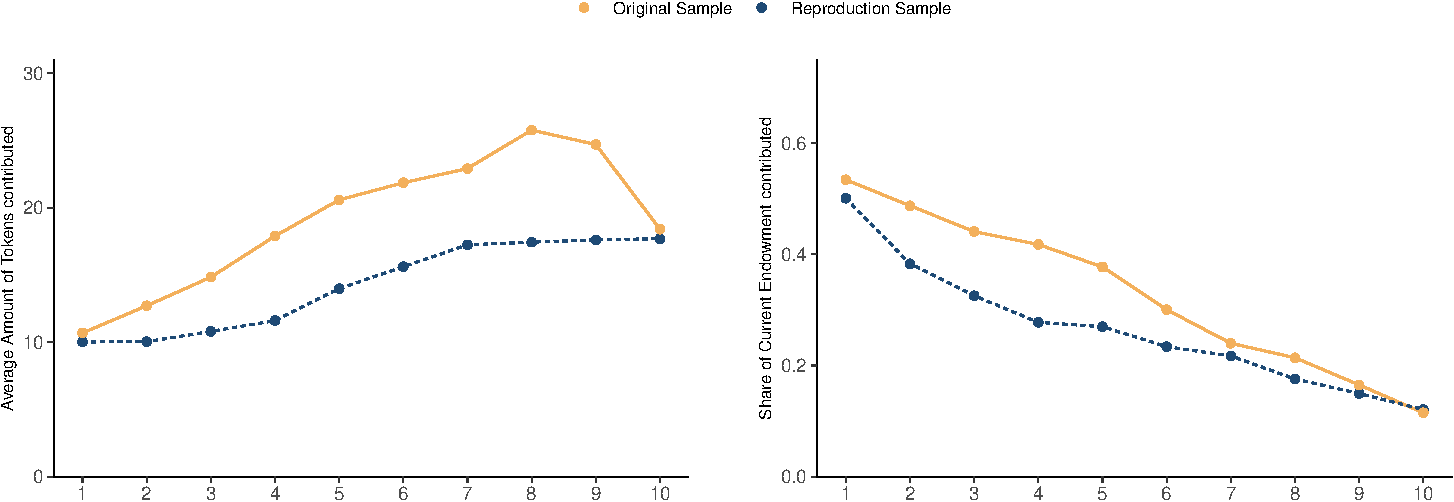
\includegraphics{paper_files/figure-pdf/fig-share-of-contributions-1.pdf}

}

\caption{\label{fig-share-of-contributions}The average amount of tokens
contributed over time in treatments.}

\end{figure}

Again, both samples' behavior resembles the contributions participants
usually make in the static game with partner matching: contributions
equal approximately half of endowments in the very first period and
decrease to around ten percent of endowments by the last
period.\footnote{The right panel is thus, comparable to the
  visualizations \emph{and results} in the static game. See, for
  instance, Figure 1B in \citet[p.986]{fehrgaechter2000}.} In the
dynamic game presented here, however, different paths lead to different
levels of wealth -- even if they share the same start- and end-points. I
am thus, more interested in the contributions' implications for wealth
generation and growth.

\hypertarget{sec-wealth}{%
\subsubsection{Wealth Creation}\label{sec-wealth}}

How do the different contribution-paths translate into
wealth?\footnote{To measure wealth and growth, I define a variable
  called \emph{stock} which sums the endowments of all participants in a
  given group at the end of the round (that is, after the contributions
  have been made, multiplied and redistributed).} Given that the
original sample contributed more, one would expect the respective groups
to be more wealthy. A mere mean comparison indicates just that: An
average group in the original sample accumulated about 478 tokens. In
contrast, an average group in the reproduction sample accumulated about
380 tokens. This difference is insignificant at conventional levels
though: A two-sided rank sum test (comparing differences between
samples) yields p=0.1356 for the mean stock in last period of the game.

Although there clearly is growth, groups do not realize the maximal
potential efficiency: under full cooperation, a group can accumulate at
least 4613 tokens or EUR 230. This is depicted in the left panel of
Figure~\ref{fig-growth-heterogeneity}, where one can see the average
wealth over time by sample. The panel illustrates for both samples that
growth was continuous and surprisingly linear, given the exponential
character of the game's design. Despite somewhat differing contribution
behavior between samples, neither the eventual wealth nor the
corresponding growth paths differed. Differences in contribution
behavior did, thus, not translate to significantly different wealth
outcomes.

Why? Perhaps because the heterogeneity within samples and across groups
has been too large to \emph{detect} a significant difference. The right
panel of Figure~\ref{fig-growth-heterogeneity} depicts heterogeneity: In
the reproduction sample, the richest group earned 1425 tokens (which is
about 1781\% of the initial endowment) whereas the poorest group ends up
with 92 tokens (115\%). More broadly, the reproduction sample is
characterized by inequality between groups (\(SD_{Replication} =\)
336.06). The same holds true for the original sample
(\(SD_{Original} =\) 393.58). Hence, the heterogeneity across groups
does not differ between samples, which is remarkable because the
reproduction sample was drawn from a more heterogeneous (non-convenience
sample). Does it differ within groups?

\begin{figure}

{\centering 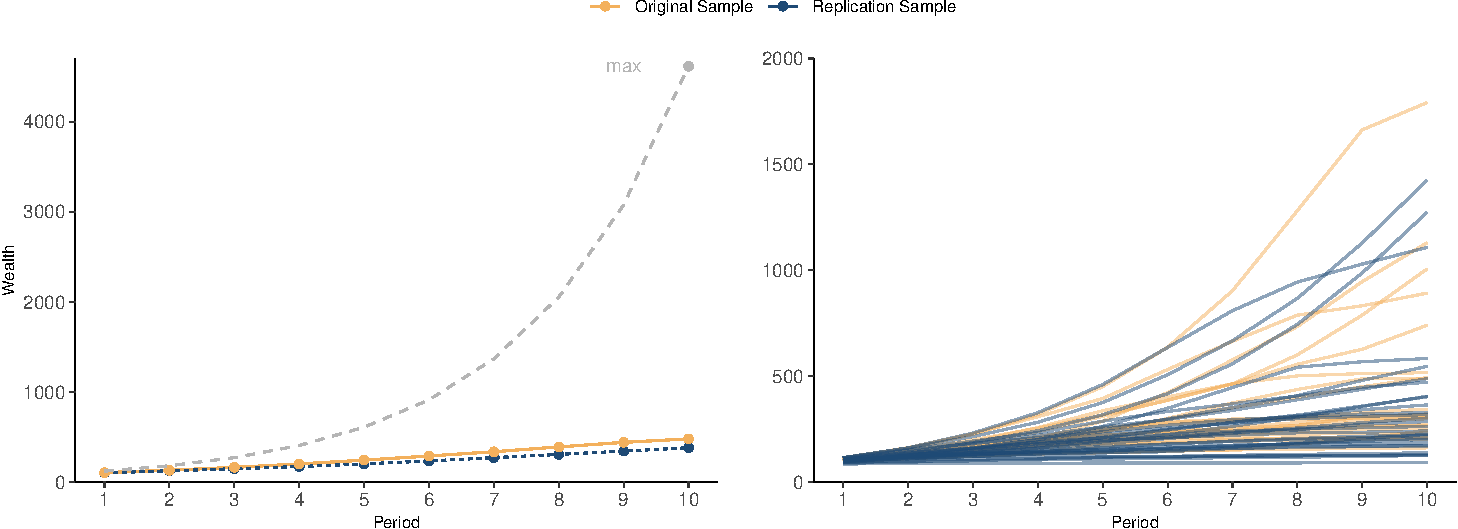
\includegraphics{paper_files/figure-pdf/fig-growth-heterogeneity-1.pdf}

}

\caption{\label{fig-growth-heterogeneity}Average wealth over time across
samples.}

\end{figure}

\hypertarget{sec-inequality}{%
\subsubsection{Inequality}\label{sec-inequality}}

Given the different samples and the possibility of endogenous
growth--which essentially is the main feature of the game--I ask whether
and how the inequality grows \emph{within} groups.
Figure~\ref{fig-gini-time-series} illustrates that inequality did grow:
at the end of the game, the original and the replication groups exhibit
an average Gini coefficient of 0.23 and 0.22, respectively.\footnote{The
  two-sided rank sum test (comparing differences between samples) yields
  p=0.6059 for the mean Gini coefficient in last round of the game.}
Because every participant started with the same initial endowment (in
\emph{period 0}, so to speak), every group started equally--with a Gini
coefficient equaling zero.

Figure~\ref{fig-gini-time-series} also shows that this initial state of
equality ended with the first period already: both samples exhibit a
stark incline in inequality before the second period started. From then
on, the respective Gini coefficients grew slowly but continuously -- for
both samples.\footnote{In each and every period, the two-sided rank sum
  test comparing gini coefficients between both sample yields p-values
  way over ten percent.}

\begin{figure}

{\centering 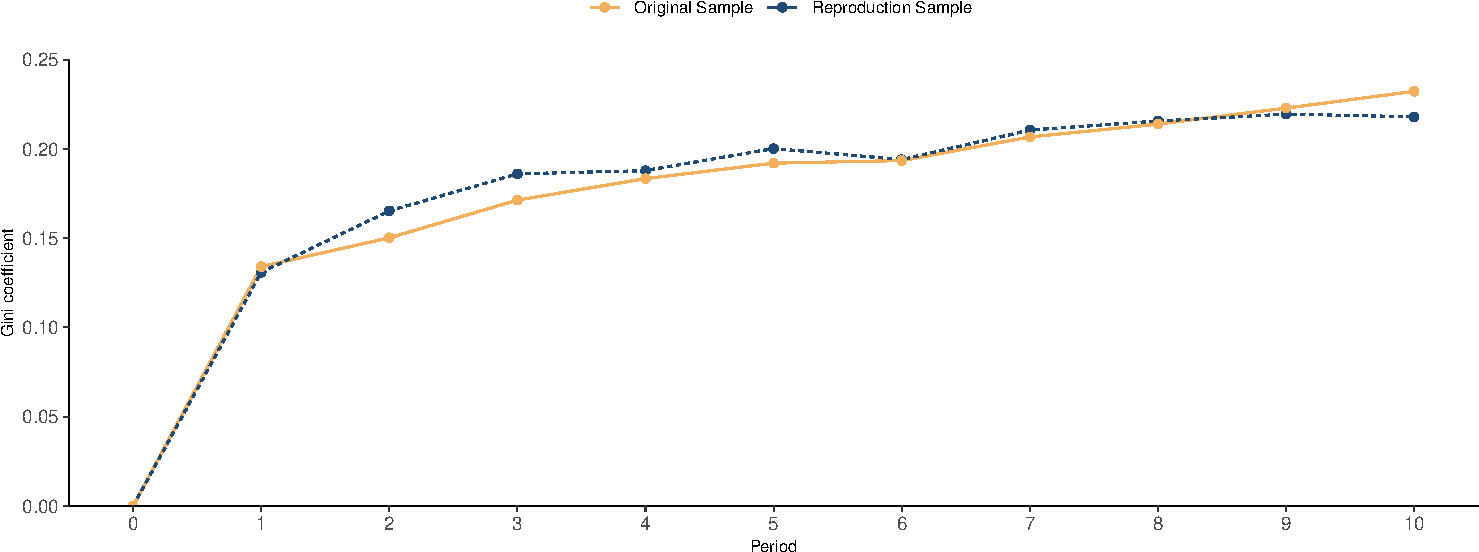
\includegraphics{paper_files/figure-pdf/fig-gini-time-series-1.pdf}

}

\caption{\label{fig-gini-time-series}Average Gini coefficient (within
groups) over time across samples}

\end{figure}

\textbf{Result 1.} \emph{The \texttt{NOPUNISH\ 10} treatment of GMTV can
be replicated because the replication data resemble the original data
with respect to initial and final contributions, wealth and growth as
well as inequality.}

This is remarkable given the different sample and language, the
different software and user interface as well as the online setting
during the COVID19 pandemic. The result suggests that, by and large, the
sum of these factors did not affect people's preferences towards
cooperation.

\hypertarget{sec-feasibility}{%
\subsection{Online Feasibility}\label{sec-feasibility}}

Throughout this section, I do not consider GMTV's data and pool data I
gathered from the citizens as well as the students from Hamburg (N =
151).

How did the participants, who have never participated in an online group
experiment before, cope with the situation? Moreover, did participants
understand the unfamiliar setting they found themselves in? While the
answer to the former question requires more thought, the answer to the
latter simply is \emph{yes}: 67 out of 116 answered with \emph{``yes''}
when I asked them. Another 44 answered with \emph{``rather yes''} while
nobody indicated that he or she did not understand the situation at all.
There is some behavioral data supporting this finding: The user
interface offered a popup to review instructions or contact information.
I tracked both and find that none of the participants ever opened these
popups even though they were clearly visible in the decision screen's
header and introduced in the instructions. To further analyze how
participants coped with the situation, I consider three additional
metrics: selection into the experiment, attrition as well as the time
spent on each page.

I first comment on the selection into the experiment: It was difficult
to recruit the sample. The panel counted 1.209 non-students of which I
were able to recruit 130 participants who finished the experiment---even
though I varied the weekdays and timing of the sessions (which were
conducted during a nation-wide lockdown with home office regime). For
this reason, I also recruited students in the last session which
explains the relatively large number of showups in Table~\ref{tbl-meta}.
Although I intended to refrain from the recruitment of students
initially, this particular sub sample enabled me to investigate the
generalizability of my results as I will discuss in
Section~\ref{sec-generalizability}.

\hypertarget{tbl-meta}{}
\begin{table}
\caption{\label{tbl-meta}The Experimental Sessions' Meta Data }\tabularnewline

\centering
\begin{tabular}{l|l|l|r|r|r|r|r}
\hline
Session Code & Date & Time & Showups & Dropouts & Residuals & Participants & Observations\\
\hline
jyf8xd0s & 2021-07-01 & 15:00 & 35 & 4 & 3 & 28 & 7\\
\hline
vggk2gh1 & 2021-07-03 & 13:00 & 20 & 8 & 0 & 12 & 3\\
\hline
8gi7c8xg & 2021-07-09 & 13:00 & 21 & 5 & 4 & 12 & 3\\
\hline
d6jrsxnr & 2021-07-23 & 14:00 & 75 & 8 & 3 & 64 & 16\\
\hline
\end{tabular}
\end{table}

Turning to the time spent on each page, I focus on the decision times in
the dynamic public goods game as \citet{Anderhub2001} did. How many
seconds did the participants need to make a decision in each period of
the game? Not too many. Figure~\ref{fig-time-spent} illustrates an
intuitive pattern: The first decision took about 22 seconds. The second
decision--where participants first learned about the other group
members' previous decisions--took longer (about 33 seconds).
Subsequently, decision times first declined and stabilized at 19
seconds. Importantly, decision times were so short that crosstalk, that
is, communication through private channels--a common concern\footnote{See,
  for instance, the discussion section in \citet[p.~119]{AGM2018}.} in
online experiments--was unlikely, especially because it would require
the identification of other group members.\footnote{There were only 9
  participants (from all four sessions) who needed more than 60 seconds
  to make the second decision.}

\begin{figure}

{\centering 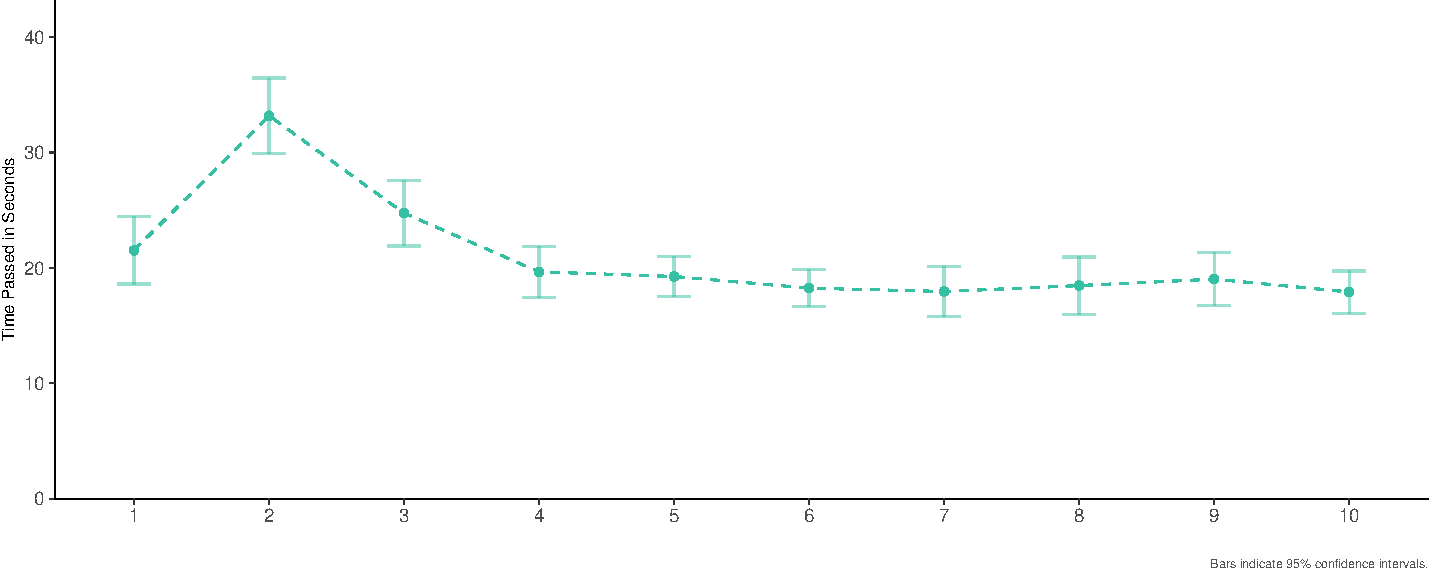
\includegraphics{paper_files/figure-pdf/fig-time-spent-1.pdf}

}

\caption{\label{fig-time-spent}Average Time Spent for each Contribution
per Period}

\end{figure}

Considering attrition, I find that it did not affect the interactive
experiment at all. To elaborate, I differentiate between dropouts and
residuals: Participants who could not be matched to other group members
are called residuals. Participants who intentionally left the experiment
are called dropouts. Residuals did not participate in the experiment
\emph{by design}. Dropouts did not participate in the experiment
\emph{by choice}. Out of 151 people who showed up, I count 10 residuals
and 25 dropouts. All of the residuals waited to be matched to a group
unsuccessfully before they got paid one Euro for their patience. In
contrast, all of the dropouts left while reading the instructions and
before being matched to other group members. Moreover, they got no
payment at all. Hence, attrition was no concern considering the dynamic
public goods game or the expenses.

\textbf{Result 2.} \emph{Given the decision times and the fluent
procedure, attrition was as negligible as it is in physical
laboratories---where (a) not every invited person shows up and (b) a
number of participants divisible by the group size is required as well.}

\hypertarget{sec-generalizability}{%
\subsection{Generalizability}\label{sec-generalizability}}

As before, I do not consider GMTVs' data in this section. Instead, I
will differentiate between data from the citizens and the students from
Hamburg. I refer to the two samples as the \emph{students} (\(N_s\) =
64) and the \emph{general population sample} (\(N_g\) = 52),
respectively.

\citet{GKLS2020} asked how much can we learn about voluntary climate
action from the behavior in public goods games. Using a similar
strategy, I answer the question for a \emph{dynamic} public goods game:
\emph{Not much}. Overall, there seems to be no association between
choices in the voluntary climate action and the first period in the
dynamic public goods game.

Figure~\ref{fig-kernel-generalizability} shows distributions of
contributions across both choices for both samples. The top panels
illustrate the behavior of the general population sample. The bottom
panels illustrate the behavior of the student sample. The left panels
show the behavior in the VCA. The right panels show the behavior in
first period of the game. A visual inspection shows that (a) mean
contributions are positive in both tasks for both samples.\footnote{The
  same holds true for median contributions.} (b) Furthermore, average
contributions are lower in the VCA. (c) In contrast to
\citet{GKLS2020}'s observation, I do not observe a difference between
samples in the abstract game's contribution behavior. (d) However, the
student's share of income contributed to the VCA is significantly lower
than the general population sample's contributions (two-sided rank sum
test, p=0.0085). Taken together, these aggregate results indicate, that
the consistency between tasks is higher for the general population than
it is for students. Or, to put it differently, the general population's
behavior in the abstract game better predicts their behavior in
real-world mitigation context.

\begin{figure}

{\centering 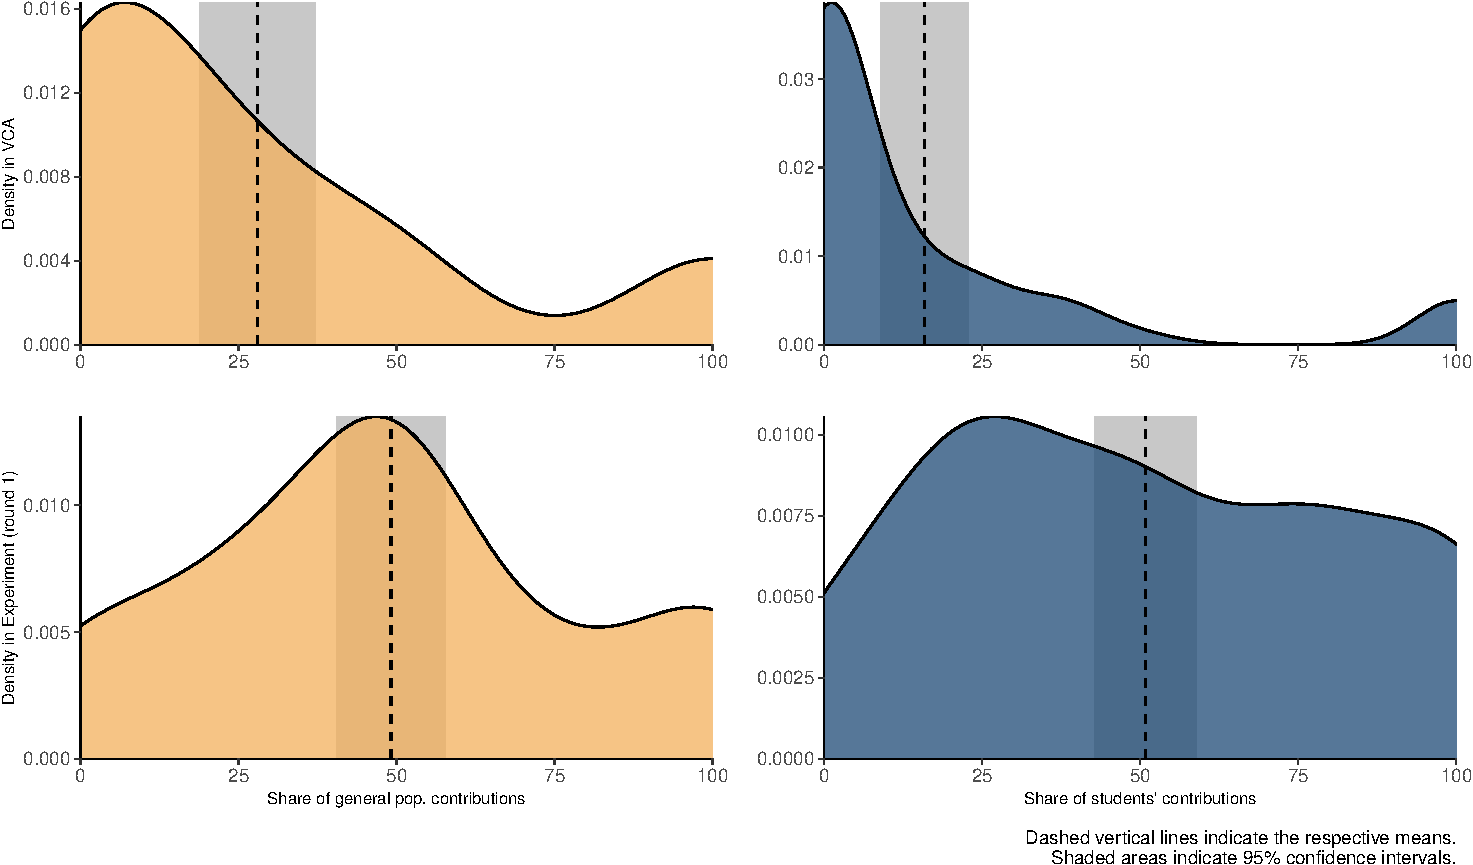
\includegraphics{paper_files/figure-pdf/fig-kernel-generalizability-1.pdf}

}

\caption{\label{fig-kernel-generalizability}Kernel distributions of
contributions across tasks and subject pools.}

\end{figure}

Table~\ref{tbl-tobit-generalizability} shows that this is not the case.
It reports tobit regression results cautioning against transferability
from dPGG results to real-world mitigation behavior: The share of
endowment contributed in the first period (displayed in the first row)
does not predict the share of earnings donated as a VCA. The student
status negatively affects VCA donations in column two but disappears if
one controls for age in column three. Importantly, the interaction of
student status and first-period contributions is not significant. This
suggests that the general population sample's transferability is just as
bad as the student sample's. I thus, find a similar result as
\citet[p.6]{GKLS2020}.

\hypertarget{tbl-tobit-generalizability}{}
\begin{table}[!htbp] \centering 
  \caption{\label{tbl-tobit-generalizability}Correlations between first-round-dPGG and VCA behavior } 
  \label{} 
\begin{tabular}{@{\extracolsep{5pt}}lccc} 
\\[-1.8ex]\hline 
\hline \\[-1.8ex] 
 & \multicolumn{3}{c}{Tobit Regression censoring below 0 and above 100} \\ 
\cline{2-4} 
\\[-1.8ex] & \multicolumn{3}{c}{VCA Donation as Share of Earnings} \\ 
\\[-1.8ex] & (1) & (2) & (3)\\ 
\hline \\[-1.8ex] 
 First-period contribution in percent & 0.07 & $-$0.17 & $-$0.23 \\ 
  & (0.18) & (0.25) & (0.25) \\ 
  & & & \\ 
 Student (1 = yes) &  & $-$48.68$^{**}$ & $-$31.06 \\ 
  &  & (20.44) & (21.74) \\ 
  & & & \\ 
 First-period contr. x Student & 4.00$^{***}$ & 3.96$^{***}$ & 3.94$^{***}$ \\ 
  & (0.11) & (0.11) & (0.11) \\ 
  & & & \\ 
 Age &  &  & 0.92$^{**}$ \\ 
  &  &  & (0.45) \\ 
  & & & \\ 
 Female (1 = yes) &  &  & 4.98 \\ 
  &  &  & (10.74) \\ 
  & & & \\ 
 Risk Aversion (1-12) &  & 0.46 & 0.50 \\ 
  &  & (0.34) & (0.34) \\ 
  & & & \\ 
 Constant & 3.16 & 29.35$^{**}$ & $-$13.93 \\ 
  & (10.70) & (14.67) & (26.41) \\ 
  & & & \\ 
\hline \\[-1.8ex] 
Observations & 116 & 116 & 116 \\ 
Log Likelihood & $-$359.78 & $-$356.07 & $-$354.01 \\ 
Akaike Inf. Crit. & 725.55 & 722.15 & 722.02 \\ 
Bayesian Inf. Crit. & 733.82 & 735.91 & 741.29 \\ 
\hline 
\hline \\[-1.8ex] 
\textit{Note:}  & \multicolumn{3}{r}{$^{*}$p$<$0.1; $^{**}$p$<$0.05; $^{***}$p$<$0.01} \\ 
\end{tabular} 
\end{table}

\textbf{Result 3.} \emph{There is no significant correlation between
average contributions in the abstract public goods game and
contributions to the real public good of climate change mitigation---for
none of the samples.}

\hypertarget{sec-conclusion}{%
\section{Conclusion}\label{sec-conclusion}}

The initial goal of the experiment was to reproduce specific experiments
of GMTV in an online setting using a general population sample. The
results suggest that it is important to reproduce experiments---both
purely and scientifically \citep[ p.~716]{Hamermesh2007}---before
drawing conclusions about generalizability.

The three most important findings are as follows: First, the
contribution behavior in my experiment is statistically similar to the
behavior reported in the original study. Consequently, the outcomes
growth and inequality are reproducible. Second, the online experiment
proceeded fluently such that dropouts were no concern. Third,
contribution behavior in the dynamic abstract setting is not linked to
behavior in the real world -- neither for students nor a more
representative sample.

The significance of the first result is that similar procedures led to
replicable findings under different circumstances across two different
samples. The second result is of methodological importance: It
highlights that even logistically complex experiments can be conducted
online with---not only with clickworkers but also with a true general
population sample. The third result questions whether recruiting from
more representative samples is worth the efforts because it did not
affect transferability of abstract results to the real world.

Limitations?

\newpage{}

\hypertarget{a-pure-replication}{%
\section{A: Pure Replication}\label{a-pure-replication}}

This section comments on two errors as well as a misconception I found
in the original data.\footnote{The data can be found in the
  supplementary materials they provide in their
  \href{https://www.sciencedirect.com/science/article/pii/S0047272717300361\#s0115}{online
  appendix}.} Before I proceed to explain this in more detail I would
like to say that the results of the original paper still hold after the
error is fixed and that the authors responded kindly and quickly,
showing an interest in solving the issue. In fact, some explanations in
this section stem from input provided by the authors.

\hypertarget{error-1-the-gini-coefficient}{%
\subsubsection{Error 1: The Gini
coefficient}\label{error-1-the-gini-coefficient}}

The Gini coefficient is wrongly computed in some periods for some group
members. The authors found that this happened whenever two group members
had exactly the same endowment because the program failed to rank these
group members for further calculations.

Table~\ref{tbl-gini-error} illustrates this problem. It shows group 101
in period 5 and documents that the Gini coefficient differs among group
members. According to the authors, the Gini coefficient should equal
\texttt{GINI=}0.127 for all subjects in the group. Instead, participant
\texttt{112} and \texttt{113} who have an equal endowment deviate from
that value. Importantly, the \texttt{DescTools::Gini()} function in the
statistical software \texttt{R} does not yield this error, which is why
I use that function for my calculations using both my as well as the
original data.

\hypertarget{tbl-gini-error}{}
\begin{table}
\caption{\label{tbl-gini-error}Subset of Data illustrating the Gini Coefficient's Error }\tabularnewline

\centering
\begin{tabular}{r|r|r|r|r|r|r|r|r|r}
\hline
exp\_num & gr\_id & per & subj\_id & tokens & other1 & other2 & other3 & gini & GINI\\
\hline
1 & 101 & 5 & 111 & 42 & 27 & 27 & 30 & 0.127 & 0.127\\
\hline
1 & 101 & 5 & 112 & 27 & 42 & 27 & 30 & 0.111 & 0.127\\
\hline
1 & 101 & 5 & 113 & 27 & 42 & 27 & 30 & 0.111 & 0.127\\
\hline
1 & 101 & 5 & 114 & 30 & 42 & 27 & 27 & 0.127 & 0.127\\
\hline
\end{tabular}
\end{table}

\hypertarget{error-2-the-share-of-endowments-contributed}{%
\subsubsection{Error 2: The share of endowments
contributed}\label{error-2-the-share-of-endowments-contributed}}

The original data provides a wrong measure of the share of endowments
contributed (\texttt{mean}) because it relies on a lagged endowment
(\texttt{gdp}). More precisely, the authors used the following STATA
code for their calculations:

\begin{verbatim}
*tsset subj_id per
*gen mean=sum/l.gdp
\end{verbatim}

Table~\ref{tbl-mean-error} reports participant 111 in group 101 in
experiment 1 over three periods. Both the \texttt{gdp} (that is, the sum
of the group's endowments at the beginning of the period) as well as the
\texttt{sum} (that is, the sum of the group's contributions) are
group-level variables.

\hypertarget{tbl-mean-error}{}
\begin{table}
\caption{\label{tbl-mean-error}Subset of Data illustrating the Means's Error }\tabularnewline

\centering
\begin{tabular}{r|r|r|r|r|r|r|r}
\hline
exp\_num & gr\_id & per & subj\_id & gdp & sum & mean & MEAN\\
\hline
1 & 101 & 4 & 111 & 116 & 18 & 0.168 & 0.155\\
\hline
1 & 101 & 5 & 111 & 126 & 18 & 0.155 & 0.143\\
\hline
1 & 101 & 6 & 111 & 136 & 17 & 0.135 & 0.125\\
\hline
\end{tabular}
\end{table}

Calculating the share as \texttt{MEAN=sum/gdp} solves the problem and
yields \(\frac{18}{126}=0.143\) in period 5. I thus, used this proposed
definition for all my calculations using both my as well as the original
data.

\hypertarget{the-misconception-timing}{%
\subsubsection{The misconception:
Timing}\label{the-misconception-timing}}

The authors wrote a note stating that the Gini coefficient as well as
the wealth in the paper always refer to the situation at the start of a
period and that they clarify this because the paper (last paragraph at
the bottom of page 5), says that wealth is defined as the endowment at
the beginning of the following period. Furthermore, they write that this
error came about as they switched between these two definitions during
the course of revising the paper.

I argue that it makes more sense to calculate the variables as they
state in the paper. More precisely, I think that the wealth at the
\emph{beginning} of a period is less interesting than the wealth at the
\emph{end} of a period for two reasons: First, there is no need for such
a variable because it already exists (the endowment). Second, this
definition yields a value that is determined by the design of the game
but misses an important outcome at the end of the game. To illustrate
this, note that the wealth would be defined as four times the initial
endowment in period 1. Also note that the very last value would equal
the wealth at the beginning of the last period and says nothing about
the outcome of that period. Because the contributions often drop in the
last period, this outcome is of particular interest (yet, not
represented in the data). Moreover, this definition of wealth yields
more informative values to calculate the Gini coefficient for the same
reasons: We know that the Gini coefficient is zero \emph{before} the
participants made any decision by design. We do no know the inequality
at the very end of the game---and the current definition does not tell
us.

For these reasons, I define wealth and inequality measures as the
outcomes of a period for all of my calculations using both my as well as
the original data.\footnote{Accordingly, the definition of \texttt{GINI}
  I provide in Table~\ref{tbl-gini-error} is not the definition I used
  to calculate the current period's Gini coefficient but the previous
  period's Gini coefficient.}

\newpage{}


  \bibliography{../biblio.bib}


\end{document}
